\section{UML Diagrams}
This section will cover the UML diagrams for the system. The UML diagrams are a visual representation of the system's architecture, design, and functionality, and help in understanding the system's structure and behavior. 

\subsection{Use Cases}
\begin{figure}[htbp]
    \centering
    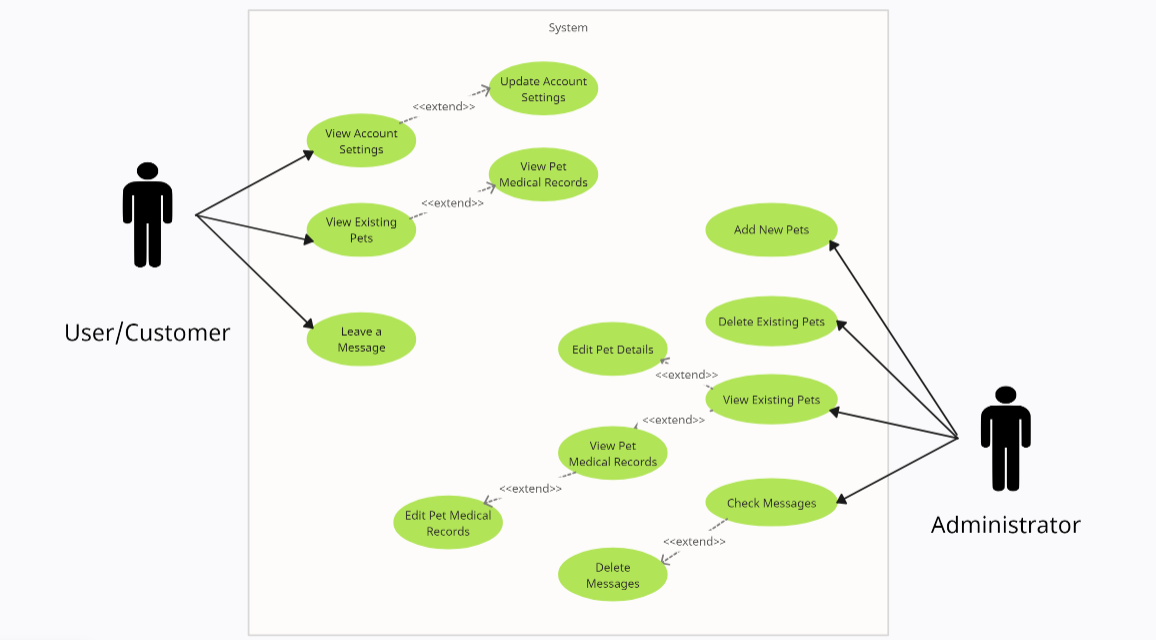
\includegraphics[width=\textwidth]{images/Use Case Diagram.png}
    \caption{Use Case Diagram showing the different use cases of the system.}
\end{figure}

The above Use Case diagram effectively incorporates the different use cases of our system and the actors involved in each use case. The actors are the admin and the user/customer. The admin add new pets, view existing pets which extends to editing their details or medical records which further extends to editing the medical records as we need to be able to manage and update pet records. The admin can also delete a pet. Admin can also check messages, which they can choose to delete. 

The user can view and update their own account, view pets, view existing pets and their details, and contact the shelter. The user can also view the shelter information.

\newpage
\subsection{Sequence Diagram}
Based on the use cases, and provided system specifications, and functional reuqirements, we have created the following sequence diagram which encapsulates the requests / responses made from the system and to the database to fetch required information based on made requests.
\begin{figure}[H]
    \centering
    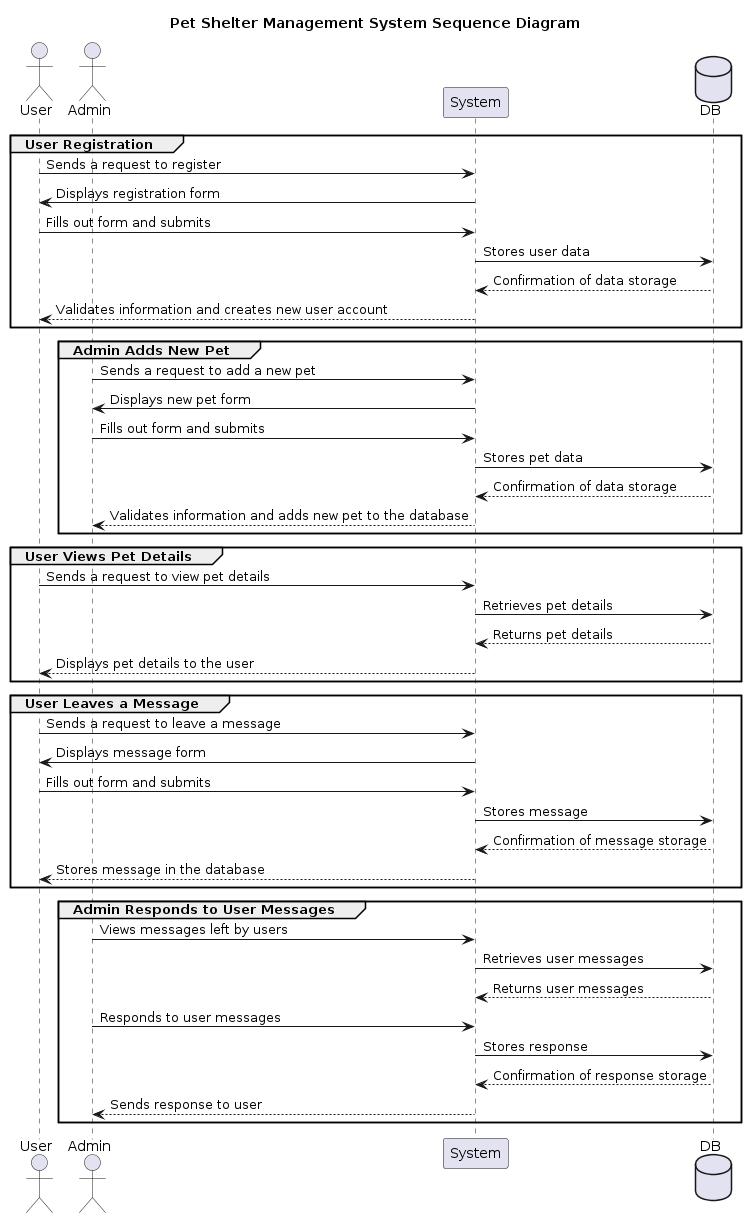
\includegraphics[width=0.7\textwidth]{images/seqDiagram.png}
    \caption{Sequence Diagram showing user/admin-system interaction}
\end{figure}


\subsection{Class Diagram}
\begin{figure}[H]
    \centering
    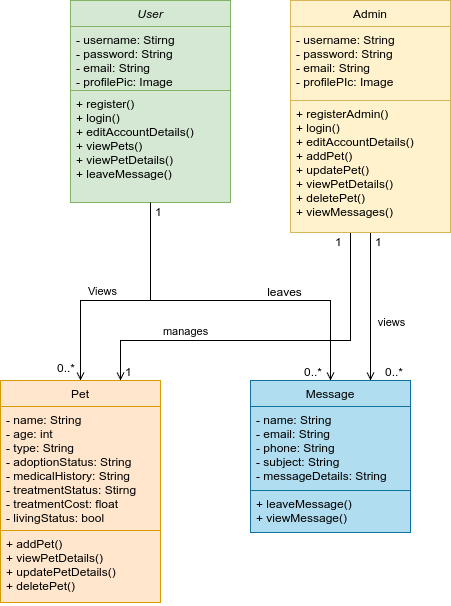
\includegraphics[width=0.8\textwidth]{images/classDiagram.png}
    \caption{Class Diagram showing the different classes and their relationships}
\end{figure}
A user can view multiple pets or a pet can be viewed by multiple users. A user can also leave multiple messages, but a message can only be left by one user. An admin can manage multiple pets, and can also respond to multiple messages.

\subsection{ERD}
\begin{figure}[H]
    \centering
    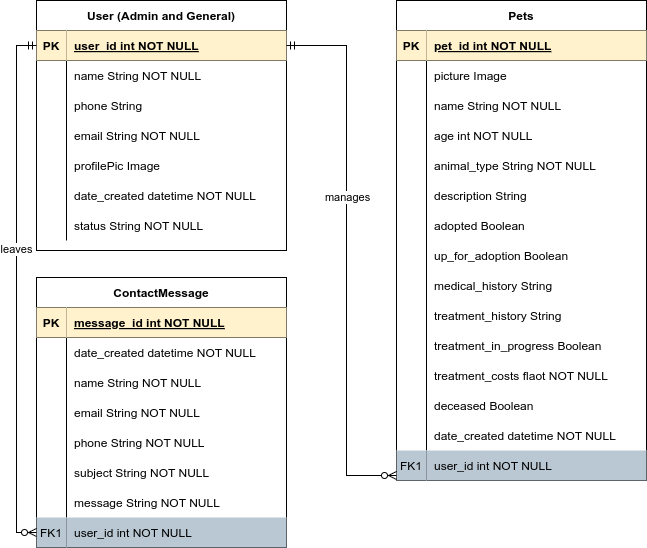
\includegraphics[width=\textwidth]{images/erd.png}
    \caption{Entity Relationship Diagram showing the different entities and their relationships}
\end{figure}
In the above ERD diagram, we represent both the general user and admin by one table since they mostly contain the same information, apart from status which basically tells if the user is an admin or not. Each user has their own unique id. Each user can leave multiple messages, however, one message belongs to only one user, hence we define a one-to-many relationship between the user and message table, with the \verb|user_id| being the foreign key in the message table. Similarly, each pet can be viewed by multiple users, however, there is no relation defined for this since it is not necessary for the system. However, one admin can manage multiple pets, hence we define a one-to-many relationship between the admin and pet table, with the \verb|user_id| being the foreign key in the pet table. Each pet also has a unique \verb|pet_id| associated with it, which is used to identify each pet and display that pet's information. 

\newpage
\subsection{Architecture}
\begin{figure}[htbp]
    \centering
    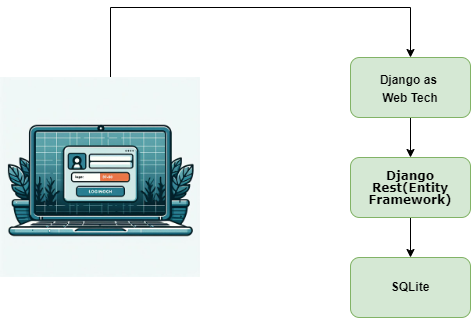
\includegraphics[width=0.85\textwidth]{images/Architecture Diagram.png}
    \caption{Architecture Diagram showing the different components of the system}
\end{figure}
Our architectural diagram is defined as shown above. We have made a web application using the python's Django as our main web technology. With Django, we've used basic HTML, CSS, and JavaScript for implementing various functionalities for the web-pages. For the API calls and handling, we've used Django Rest Framework which is a powerful and flexible toolkit for building Web APIs, efficiently handling the requests and responses. Our data is being stored in a SQLite database, a lightweight file based database which is easy to use and manage. 

%%%%%%%%%%% Sequence Diagram PlantUML Script %%%%%%%%%%%
% @startuml
% actor User
% actor Admin
% participant System
% database DB

% title Pet Shelter Management System Sequence Diagram

% group User Registration
% User -> System : Sends a request to register
% System -> User : Displays registration form
% User -> System : Fills out form and submits
% System -> DB : Stores user data
% DB --> System : Confirmation of data storage
% System --> User : Validates information and creates new user account
% end

% group Admin Adds New Pet
% Admin -> System : Sends a request to add a new pet
% System -> Admin : Displays new pet form
% Admin -> System : Fills out form and submits
% System -> DB : Stores pet data
% DB --> System : Confirmation of data storage
% System --> Admin : Validates information and adds new pet to the database
% end

% group User Views Pet Details
% User -> System : Sends a request to view pet details
% System -> DB : Retrieves pet details
% DB --> System : Returns pet details
% System --> User : Displays pet details to the user
% end

% group User Leaves a Message
% User -> System : Sends a request to leave a message
% System -> User : Displays message form
% User -> System : Fills out form and submits
% System -> DB : Stores message
% DB --> System : Confirmation of message storage
% System --> User : Stores message in the database
% end

% group Admin Responds to User Messages
% Admin -> System : Views messages left by users
% System -> DB : Retrieves user messages
% DB --> System : Returns user messages
% Admin -> System : Responds to user messages
% System -> DB : Stores response
% DB --> System : Confirmation of response storage
% System --> Admin : Sends response to user
% end
% @enduml